\documentclass{article}


\usepackage{preamble}

\title{Error Correcting Codes, Hardness Amplification and Boosting.}
\date{}

\begin{document}
    
\noindent Error Correcting Codes, Hardness Amplification and Boosting \hfill  CS 250, Winter 2025\\
\hrule

\section{Introduction}

\section{Preliminaries}

\section{Hardness Amplification with ECCs}

\begin{definition}{3.x}
    We say that a function $G : \pmo^\ell \rightarrow \pmo^{n}$ is an $(\ell, n)$-PRG if, for any size $n$ circuit $C$ over $n$ inputs, 
    \begin{equation*}
        \left|\Pr_{x \backsim U_n}[C(x)] - \Pr_{x \backsim U_s}[C(G(s))]\right| < \frac{1}{10}.
    \end{equation*}
\end{definition}

The parameter $\ell$ is the seed length.

\begin{assumption}{1} \label{a-1}
    There exists a function $f : \pmon \rightarrow \pmo$ such that $f$ can be computed in time $2^{O(n)}$, but there exists some $\delta > 0$ such that 
    \begin{equation*}
        \Corr\left(f, 2^{\delta n}\right) < 1.
    \end{equation*}
\end{assumption}

\begin{assumption}{2} \label{a-2}
    There exists a function $f : \pmon \rightarrow \pmo$ such that $f$ can be computed in time $2^{O(n)}$, but there exists some $\delta > 0$ such that 
    \begin{equation*}
        \Corr\left(f, 2^{\delta n}\right) < 2^{-\Omega(n)}.
    \end{equation*}
\end{assumption}

We will prove that, given a worst case hard function $f$, we can transform it into an average case $f'$.

\begin{theorem}{3.x} If there exists a function $f$ satisfying the worst case hardness assumption, there exists a function $f'$ satisfying the average case hardness assumption.

\end{theorem}

\subsection{Why Hardness Amplification?}

\begin{theorem}{3.x} Suppose that $G$ is a $(O(\log n), n)$-PRG computable in $\poly(n)$ time. Then $\P = \BPP$.
\end{theorem}

\subsubsection{A Simple PRG}

\begin{theorem}{3.x}
    Given the average case hardness assumption, there exists a $(n - 1, n)$-PRG.
\end{theorem}

\subsubsection{The Nisan-Wigderson Generator}

\begin{theorem}{3.x}
    Given the average case hardness assumption, there exists a $(O(\log n), n)$-PRG.
\end{theorem}

\begin{center}
    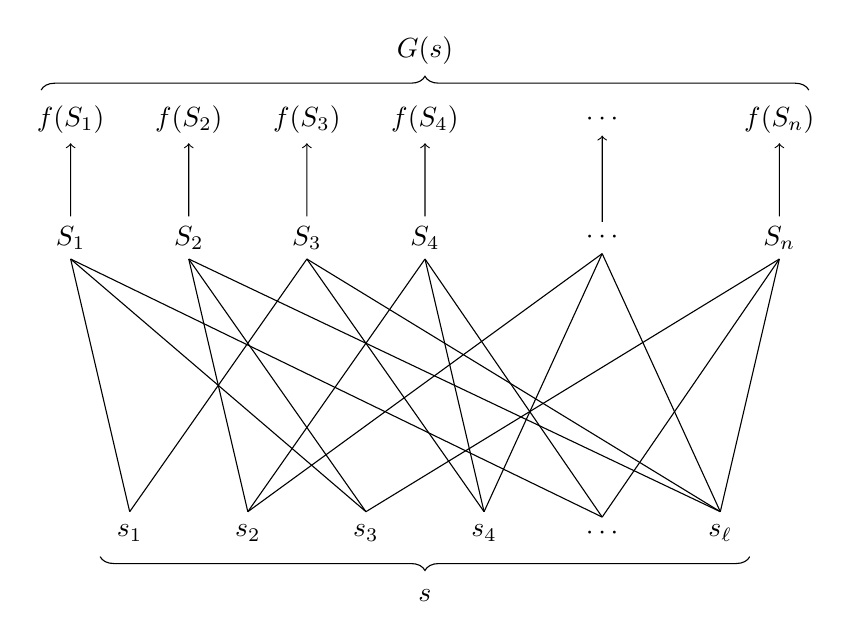
\begin{tikzpicture}[align=center,node distance=4cm, scale=1.5]
        \node[circle, inner sep=0pt, minimum size=15pt] (1) at (1, 0) {$s_1$}; 
        \node[circle, inner sep=0pt, minimum size=15pt] (2) at (2, 0) {$s_2$};
        \node[circle, inner sep=0pt, minimum size=15pt] (3) at (3, 0) {$s_3$};
        \node[circle, inner sep=0pt, minimum size=15pt] (4) at (4, 0) {$s_4$};
        \node[] (5) at (5, 0) {$\cdots$};
        \node[circle, inner sep=0pt, minimum size=15pt] (6) at (6, 0) {$s_{\ell}$};

        \node[] (11) at (.5, 2.5) {$S_1$};
        \draw[] (1.north) -- (11.south);
        \draw[] (3.north) -- (11.south);
        \draw[] (5.north) -- (11.south);

        \node[] (21) at (.5, 3.5) {$f(S_1)$};

        \draw[->] (11) -- (21);


        \node[] (12) at (1.5, 2.5) {$S_2$};
        \draw[] (2.north) -- (12.south);
        \draw[] (3.north) -- (12.south);
        \draw[] (6.north) -- (12.south);

        \node[] (22) at (1.5, 3.5) {$f(S_2)$};

        \draw[->] (12) -- (22);


        \node[] (13) at (2.5, 2.5) {$S_3$};
        \draw[] (1.north) -- (13.south);
        \draw[] (4.north) -- (13.south);
        \draw[] (6.north) -- (13.south);

        \node[] (23) at (2.5, 3.5) {$f(S_3)$};

        \draw[->] (13) -- (23);


        \node[] (14) at (3.5, 2.5) {$S_4$};
        \draw[] (2.north) -- (14.south);
        \draw[] (4.north) -- (14.south);
        \draw[] (5.north) -- (14.south);

        \node[] (24) at (3.5, 3.5) {$f(S_4)$};

        \draw[->] (14) -- (24);


        \node[] (15) at (5, 2.5) {$\cdots$};
        \draw[] (4.north) -- (15.south);
        \draw[] (2.north) -- (15.south);
        \draw[] (6.north) -- (15.south);

        \node[] (25) at (5, 3.5) {$\cdots$};

        \draw[->] (15) -- (25);

        \node[] (16) at (6.5, 2.5) {$S_n$};
        \draw[] (3.north) -- (16.south);
        \draw[] (5.north) -- (16.south);
        \draw[] (6.north) -- (16.south);

        \node[] (26) at (6.5, 3.5) {$f(S_n)$};

        \draw[->] (16) -- (26);

        \draw [decorate,decoration={brace,amplitude=5pt}]
  (0.25,3.75) -- (6.75,3.75) node[midway, yshift=.5cm]{$G(s)$};

        \draw[decorate, decoration={brace,amplitude=5pt, mirror}] 
        (.75, -.2) -- (6.25, -.2) node[midway, yshift=-.5cm]{$s$};
    \end{tikzpicture}
\end{center}

\subsection{Worst to Average Case Hardness}

\begin{theorem}{3.x}
    The average case hardness assumption implies the worst case hardness assumption.
\end{theorem}

\begin{center}
    \begin{tikzpicture}
        \draw[] (-.1, -1.5) rectangle (.1, 1.5);
        \node[fill=white] at (0, 1.7) {$x$};

        \draw[] (1.9, -2) rectangle (2.1, 2);


        \draw[] (3.9, -2.5) rectangle (4.1, 2.5);
    \end{tikzpicture}
\end{center}

\section{Boosting and Hardness Amplification}

\subsection{Smooth Boosters and The Hardcore Theorem}

\begin{center}
    \begin{tikzpicture}
        \path[draw] (-6.5, -2) rectangle (-2.5, 2);
        \path[draw,use Hobby shortcut,closed=true, pattern=north east lines]
        (-4,.3) .. (-4.4,.4) .. (-5.6, -.3);
        \node[fill=white] at (-4.6, -.5) {$H_1$};
        \node[] at (-4.5, 2.35) {$C_1$};


        \path[draw] (-2, -2) rectangle (2, 2);
        \path[draw,use Hobby shortcut,closed=true, pattern=north east lines]
        (0,.3) .. (.4,1) .. (.6,1.6) .. (1.4,1.4) .. (1.6, .3);
        \node[fill=white] at (.9, .7) {$H_2$};
        \node[] at (0, 2.35) {$C_2$};

        \path[draw] (2.5, -2) rectangle (6.5, 2);
        \path[draw,use Hobby shortcut,closed=true, pattern=north east lines]
        (4,.3) .. (4.4,.5) .. (5.6, -.3);
        \node[fill=white] at (4.7, -.3) {$H_3$};
        \node[] at (4.5, 2.35) {$C_3$};

        \draw[decorate, decoration={brace,amplitude=5pt, mirror}] 
        (-6.75, -2.25) -- (6.75, -2.25) node[midway, yshift=-.5cm]{};

        \draw[->] (0, -2.4) -- (0, -2.8);

        \path[draw] (-2, -7) rectangle (2, -3);
        \path[draw,use Hobby shortcut,closed=true, pattern=north east lines]
        (-.1,-5) .. (.4,-4.4) .. (1.6, -4.7);
        \node[fill=white] at (.8, -5) {$H$};
    \end{tikzpicture}
\end{center}

\subsection{Boosting via the XOR Lemma}

\section{One Shot Boosting with ECCs}


\end{document}